\IfFileExists{elsarticle.cls}{%
\documentclass[preprint,12pt]{elsarticle}
\newif\ifuseelsevier
\useelseviertrue
}{%
\documentclass[12pt]{article}
\newif\ifuseelsevier
\useelsevierfalse
}
\usepackage[utf8]{inputenc}
\usepackage[T1]{fontenc}
\usepackage{lmodern}
\usepackage{hyperref}
\hypersetup{hidelinks}
\usepackage{amsmath,amssymb}
\usepackage{booktabs}
\usepackage{longtable}
\usepackage{array}
\usepackage{graphicx}
\graphicspath{{figures/}}
\emergencystretch=3em

\begin{document}
\ifuseelsevier
\begin{frontmatter}
\title{When Is Reinforcement Learning Warranted in a Supply Chain DES? Decision-Rights Eligibility, Comparator Design, and Oracle-to-Policy Conversion}
\begin{abstract}
Reinforcement learning (RL) is often introduced into a discrete-event simulation once an action can be varied, without first establishing that the action exposes observable and resource-adjusted state-contingent value. We develop a preregistered eligibility framework comprising physical liveness, action-ranking diversity, perfect-information headroom, observable conversion, resource equivalence, and out-of-sample robustness. The framework is evaluated in a thesis-grounded reconstruction of a 13-operation military food supply chain and in disclosed convoy, readiness, and spatial extensions. A PPO advantage of $+0.000486$ against a restricted static frontier reverses against a same-contract constant: PPO minus static ReT is $-0.000018049$, CI95 $[-0.000028615,-0.000008087]$. A finite-convoy oracle later exposes material clairvoyant headroom ($+0.02212$), but ten MaskablePPO seeds convert essentially none of it. In a terminal spatial audit on 400 locked tapes, blind alternation beats cover, MPC, and depth-3 trees on order ReT, quantity-weighted ReT, attended orders, worst-node fill, and unfulfilled rations. Metric triangulation further shows that a Cobb--Douglas-inspired aggregate can reverse policy rankings while worsening spatial continuity. The evidence demonstrates that physical authority and clairvoyant headroom are insufficient to warrant RL; comparator rights, deployable information, resource accounting, and the resilience functional jointly determine whether adaptive-control claims are identified.
\end{abstract}
\begin{keyword}
Supply chain resilience \sep reinforcement learning \sep discrete-event simulation \sep static benchmark \sep comparator design
\end{keyword}
\end{frontmatter}
\else
\title{When Is Reinforcement Learning Warranted in a Supply Chain DES? Decision-Rights Eligibility, Comparator Design, and Oracle-to-Policy Conversion}
\author{}
\date{}
\maketitle
\begin{abstract}
Reinforcement learning (RL) is often introduced into a discrete-event simulation once an action can be varied, without first establishing that the action exposes observable and resource-adjusted state-contingent value. We develop a preregistered eligibility framework comprising physical liveness, action-ranking diversity, perfect-information headroom, observable conversion, resource equivalence, and out-of-sample robustness. The framework is evaluated in a thesis-grounded reconstruction of a 13-operation military food supply chain and in disclosed convoy, readiness, and spatial extensions. A PPO advantage of $+0.000486$ against a restricted static frontier reverses against a same-contract constant: PPO minus static ReT is $-0.000018049$, CI95 $[-0.000028615,-0.000008087]$. A finite-convoy oracle later exposes material clairvoyant headroom ($+0.02212$), but ten MaskablePPO seeds convert essentially none of it. In a terminal spatial audit on 400 locked tapes, blind alternation beats cover, MPC, and depth-3 trees on order ReT, quantity-weighted ReT, attended orders, worst-node fill, and unfulfilled rations. Metric triangulation further shows that a Cobb--Douglas-inspired aggregate can reverse policy rankings while worsening spatial continuity. The evidence demonstrates that physical authority and clairvoyant headroom are insufficient to warrant RL; comparator rights, deployable information, resource accounting, and the resilience functional jointly determine whether adaptive-control claims are identified.
\end{abstract}
\fi

\hypertarget{1-introduction}{%
\section{1. Introduction}\label{1-introduction}}

Supply chain resilience (SCRES) has become a central concern in
operations management as global disruptions-\/-\/-from pandemic-driven
shutdowns to geopolitical trade barriers-\/-\/-expose the fragility of
interconnected logistics networks \cite{ponomarov2009understanding,wieland2021two,hosseini2019review}. Over the past decade, reinforcement
learning (RL) has emerged as a promising paradigm for adaptive
decision-making in supply chain management (SCM). Comprehensive reviews
by Yan et al.~\cite{yan2022} and Rolf et al.~\cite{rolf2023} document a growing body of
work applying RL to inventory ordering, transportation scheduling, and
multi-echelon coordination, while Boute et al.~\cite{boute2022} provide a design
roadmap for deep RL in inventory control. More recent DES+ML reviews,
including Kogler and Maxera~\cite{kogler2026}, document papers combining discrete-event simulation (DES) with
machine learning, confirming that DES+RL is now the dominant hybrid
paradigm for operational supply chain analysis. This paper therefore
does not claim novelty in the idea of applying RL to supply chains;
instead, it contributes a benchmark-centered investigation of
\emph{when} RL works and \emph{when} it fails in resilience-oriented
operational control.

Despite this maturation, most published RL-for-SCM work concentrates on
inventory cost optimization in stylized or generic environments
\cite{gijsbrechts2022,demoor2022,dehaybe2024,geevers2024}, while the few papers addressing resilience operate
at the level of network reconfiguration rather than operational control.
Ding et al.~\cite{ding2026} represent the closest resilience competitor: they use
multi-agent PPO (MAPPO) for dynamic reconfiguration of a supply chain
system-of-systems under disruption risks, with macro-level actions such
as filling, repairing, and recruiting disrupted nodes. However, their
problem is strategic topology redesign on an abstract network,
fundamentally different from the weekly operational control-\/-\/-over
assembly shifts, inventory quantities, and transport dispatch-\/-\/-that
characterizes our setting. The gap addressed here is not whether RL can
be applied to supply chains, but whether RL can deliver resilient
operational control inside a thesis-grounded military supply chain whose
structural bottlenecks are explicitly modeled.

This work builds directly on the research agenda of Garrido-Rios~\cite{garrido2017}
and Garrido et al.~\cite{garrido2024ijpr,garrido2024iccl}. The PhD thesis developed a
13-operation military food supply chain (MFSC) simulation in
MATLAB/Simulink, establishing quantitative resilience metrics
(Re\$\^{}T\$) through 90 static configurations and data-mining
association rules. Garrido et al.~\cite{garrido2024ijpr} subsequently proposed a
Cobb-\/-Douglas factory resilience index linking production strategies
to quantitative resilience measurement. Garrido et al.~\cite{garrido2024iccl}
explicitly called for the integration of AI algorithms-\/-\/-identifying
neural networks, KANs, and reinforcement learning as the most suitable
candidates-\/-\/-into simulation-based SCRES models, arguing that
traditional DES frameworks lack endogenous learning mechanisms capable
of adaptation across successive disruption events. The present study
operationalizes this proposal: we rebuild the thesis DES in
Python/SimPy, validate it against the original reference targets
(\$-4.43\%\$ relative gap), wrap it in a Gymnasium-compatible interface,
and apply PPO-based RL control.

Our core empirical finding is dual. Under Track A---the
thesis-faithful control contract where the agent controls upstream
inventory and assembly shifts---dense common-random-number static
frontiers and multiple RL configurations across reward modes,
observation versions, and algorithms (including PPO and RecurrentPPO)
leave no publishable dynamic-control advantage: no tested learner
converts the small measured headroom over the best static policy. Under
Track B---an operational extension that adds downstream transport
dispatch control at Op10 and Op12 (an 8-dimensional action contract)
while preserving the DES backbone---PPO improves Garrido/Excel
resilience (ReT) by 0.000426 (95\% CI entirely positive) over the best
of a dense grid of 147 static dispatch comparators under paired
common-random-number evaluation, with matching gains in service
continuity and recovery-tail metrics. A 5-seed action-space ablation
shows the gain concentrates in downstream-dispatch access specifically
rather than in the number of controllable dimensions; the advantage
holds across current and increased Garrido-native risk levels at both
evaluated horizons, is mixed under severe risk; and
two independent tests rule out that the effect depends on the learned
policy exploiting privileged simulator observation fields unavailable
to static comparators. The paper's central argument is therefore
structural: RL success in this benchmark depends not on algorithmic
sophistication or reward engineering, but on whether the controllable
action space reaches the binding operational bottleneck.

The paper makes four contributions. First, we report a negative
empirical benchmark result: under the thesis-faithful action
contract, dense-frontier evaluation finds no publishable dynamic-control
advantage for learned policies. Second, we report a positive empirical
benchmark result: an operational action-space extension produces a
robust, adversarially-tested RL advantage under paired dense-frontier
evaluation. Third, we provide a structural diagnosis supported by a
causal ablation and two privileged-observation tests: the downstream
control dimensions, not action-space size or access to simulator
internals, explain the observed improvement. Fourth, we contribute a
reproducible benchmark with auditable artifacts, frozen contracts, and a
Garrido-compatible resilience evaluation pipeline. We do not claim to be
the first paper on RL for supply chains, the first DES+RL study, or to
offer architectural novelty; our contribution is experimental and
diagnostic. The remainder of the paper is organized as follows: Section
2 reviews related work across four blocks; Section 3 presents the
methodology; Section 4 reports results; Section 5 discusses implications
and limitations; and Section 6 concludes.

\hypertarget{2-related-work}{%
\section{Related Work}\label{2-related-work}}

\hypertarget{21-scres-measurement-and-adaptive-capability}{%
\subsection{SCRES measurement and adaptive capability}\label{21-scres-measurement-and-adaptive-capability}}

Supply chain resilience (SCRES) is commonly defined around the ability of
a supply chain to prepare for, respond to, and recover from disruptions
\cite{ponomarov2009understanding}. More recent theory distinguishes
resilience as a system property from resilience as a dynamic capability
that must be renewed through experience and organizational learning
\cite{wieland2021two,levitt1988organizational}. Quantitative SCRES
research has consequently moved beyond binary disruption survival toward
metrics for recovery speed, service continuity, tail performance, and
system viability \cite{hosseini2019review}. This paper follows that
measurement tradition: reinforcement learning is evaluated on
Garrido/Excel ReT and order-level recovery metrics, not on the training
reward alone.

\hypertarget{22-garrido-grounded-des-for-resilience}{%
\subsection{Garrido-grounded DES for resilience}\label{22-garrido-grounded-des-for-resilience}}

Garrido-Rios~\cite{garrido2017} provides an unusually useful starting
point for AI-enabled SCRES because the military food supply chain is
already modeled as a detailed 13-operation simulation with resilience
indices, risk families, and static policy comparisons. Garrido et
al.~\cite{garrido2024ijpr} extend that lineage through a
Cobb--Douglas-style factory resilience index, while Garrido et
al.~\cite{garrido2024iccl} explicitly identify learning algorithms as a
future path for simulation-based SCRES models. The present study answers
a narrower and more testable version of that agenda: not whether AI can
be attached to a DES, but whether learned closed-loop control can beat
strong static resilience baselines when the controllable decision surface
does or does not reach the operational recovery bottleneck.

\hypertarget{23-rl-for-supply-chain-operational-control}{%
\subsection{RL for supply-chain operational control}\label{23-rl-for-supply-chain-operational-control}}

Reinforcement learning has become an established paradigm for adaptive
decision-making in supply chain management. Yan et al.~\cite{yan2022}
and Rolf et al.~\cite{rolf2023} review applications across inventory
ordering, vehicle routing, warehouse operations, and multi-echelon
coordination. Boute et al.~\cite{boute2022} provide a design roadmap for
deep RL in inventory control, and Powell~\cite{powell2022} cautions that
neural value-function approximation is only one policy class among
several structured alternatives. Empirical inventory-control studies
reinforce that warning: deep RL can perform well, but strong base-stock,
teacher, and heuristic policies remain difficult comparators
\cite{gijsbrechts2022,demoor2022,dehaybe2024,geevers2024,temizoz2025,vanvuchelen2025}.
Our contribution is therefore not the generic application of PPO to a
supply chain. It is a controlled benchmark showing that action-surface
design can decide whether any learned policy has a useful recovery
frontier to exploit.

\hypertarget{24-des-ml-and-ai-scres}{%
\subsection{DES+ML and AI-SCRES workflows}\label{24-des-ml-and-ai-scres}}

Hybrid simulation and machine-learning workflows are now common in
supply-chain analysis. Kogler and Maxera~\cite{kogler2026} review 72
papers and 43 related studies combining discrete simulation with machine
learning, while Perez-Pena et al.~\cite{perezpena2025} show that many
simulation-ML workflows emphasize prediction or classification rather
than optimization. In resilience-oriented AI, Ding et al.~\cite{ding2026}
use MAPPO for strategic topology reconfiguration under disruption,
Bussieweke et al.~\cite{bussieweke2024recovery} combine system dynamics
and RL for recovery policies, Kim~\cite{kim2024} studies cooperative
MARL for inventory transshipment, Liu et al.~\cite{liu2025pom} apply
HAPPO to decentralized multi-echelon inventory, and Kotecha and del Rio
Chanona~\cite{kotecha2025} combine graph neural networks with MAPPO.
Other AI-SCRES studies focus on prediction, classification, or
explanation rather than online control
\cite{rajagopal2024,rezki2024,ordibazar2022}. These streams establish
the relevance of AI for SCRES, but they rarely test learned control
against dense static frontiers on a thesis-grounded resilience metric.

\begin{table}[htbp]
\centering
\caption{Positioning of the present benchmark relative to adjacent literatures.}
\label{tab:literature_gap}
\begin{tabular}{p{0.25\linewidth}ccccc}
\toprule
Stream & Validated DES & SCRES metric & Dense static frontier & Bottleneck action test & Privileged-observation defense \\
\midrule
DES SCRES models & Yes & Yes & Sometimes & Rare & No \\
RL inventory/control & Rare & No & Sometimes & Rare & Rare \\
DES+ML supply-chain workflows & Sometimes & Rare & Rare & Rare & Rare \\
AI-SCRES / MARL reconfiguration & Sometimes & Sometimes & Rare & Strategic & Rare \\
This paper & Yes & Yes & Yes & Yes & Yes \\
\bottomrule
\end{tabular}
\end{table}

\hypertarget{25-gap-action-space-alignment}{%
\subsection{Gap: action-space alignment and bottleneck authority}\label{25-gap-action-space-alignment}}

The gap is therefore conditional rather than categorical. Prior work
shows that RL can be used in supply chains and that DES can represent
SCRES dynamics. What remains under-tested is whether the learned policy's
action space actually reaches the constraint that governs recovery.
Theory-of-Constraints reasoning treats the binding bottleneck as the
lever that determines system throughput \cite{goldratt1984goal}; RL
agent design determines whether that lever is even available to the
policy. This paper connects the two: Track A tests learned control when
the original buffer/shift surface leaves the downstream recovery
bottleneck mostly fixed, while Track B tests a DES-preserving extension
that exposes downstream dispatch authority. The contribution is a
benchmark-centered diagnosis of when AI-enabled SCRES control has a
convertible recovery frontier and when it does not.

\section{Decision-right eligibility framework}\label{sec:framework}

The methodological premise is that an available action is not automatically a useful
sequential decision. Let $S_t$ denote the physical state, $O_t$ the information available to
an operator, $A_t$ an admissible action, and $J$ an episode-level resilience outcome. For a
fixed horizon $H$, define $Q_H(s,a)=\mathbb{E}[J_{t:t+H}\mid S_t=s,A_t=a]$. The value of
perfect information over the best constant action is
\begin{equation}
H_{\mathrm{PI}}=\mathbb{E}_{S}\left[\max_a Q_H(S,a)\right]
-\max_a\mathbb{E}_{S}[Q_H(S,a)].
\end{equation}
The corresponding observable value replaces the true state by the operator's information:
\begin{equation}
H_{\mathrm{obs}}=\mathbb{E}_{O}\left[\max_a\mathbb{E}[Q_H(S,a)\mid O]\right]
-\max_a\mathbb{E}_{S}[Q_H(S,a)].
\end{equation}
These quantities separate two questions often conflated in simulation--RL studies. An oracle
may profit from knowing a future disruption, while a deployable controller cannot infer the
relevant action ranking from contemporaneous observations. In that case $H_{\mathrm{PI}}>0$
but $H_{\mathrm{obs}}\approx0$; further optimization of a learner cannot manufacture the
missing information.

We operationalize eligibility as a six-stage ladder. \emph{Physical liveness} requires that
two admissible actions produce different physical trajectories under exact replay.
\emph{Ranking diversity} requires that the preferred action changes across a material fraction
of states; otherwise a constant posture is sufficient. \emph{Oracle headroom} requires a
positive and practically material paired outcome over a same-contract static comparator.
\emph{Observable convertibility} requires a policy using only deployable fields to recover
value in rollout, rather than merely classify oracle actions accurately. \emph{Resource
equivalence} requires the apparent gain to survive equal decision rights and an explicit
budget envelope. Finally, \emph{robustness} requires confirmation on frozen, previously
unopened tapes and guardrails for service, lost orders, and tail outcomes. Failure at an
earlier stage blocks claims at every later stage.

The comparator contract is central. If an RL policy controls eight variables while the static
frontier varies only three, the contrast estimates a mixture of adaptation and additional
authority. The correct static bar is the strongest implementable constant or open-loop doctrine
with the same action rights and no greater resource use. Calibration selects the comparator
once; evaluation does not reselect it per tape. Common random numbers then pair demand,
processing, repair, and disruption realizations across policies. This design turns differences
into action effects rather than differences in exogenous luck.

Observable conversion is evaluated by rollout value, not action accuracy. Suppose an oracle
labels action $a^*(s)$. A classifier minimizes $\mathbf{1}\{\hat a\ne a^*\}$, assigning equal
weight to harmless and catastrophic mistakes. The decision-relevant loss is instead regret,
\begin{equation}
\mathcal{L}_{\mathrm{regret}}(s,\hat a)=Q_H(s,a^*)-Q_H(s,\hat a),
\end{equation}
and the decisive endpoint remains episode performance against the frozen comparator. This
distinction became empirically important: a high oracle-action classification rate did not
translate into a useful sequential policy.

The framework also separates metric constructs. Order-level ReT treats continuity and lateness
per order; quantity-weighted ReT weights the same order scores by ration demand; service-loss
measures physical unmet mass; worst-node fill exposes spatial sacrifice; and a multiplicative
Cobb--Douglas index encodes a preference over inventory, backlog, time, capacity, and resource
dimensions. None is a neutral synonym for ``resilience.'' A policy-ranking reversal across
these measures is reported as construct sensitivity, not resolved by choosing retrospectively
the metric on which a learner wins.

Preregistration makes the ladder falsifiable. Each program freezes its action contract, tapes,
estimand, comparator, practical threshold, and stop rule before observing the relevant data.
A failed gate is retained as a boundary result. New physics or a new information contract
requires a separately named study and cannot alter the earlier verdict. This discipline is
particularly important when environment design itself can create or destroy learnability.


\section{Military food supply-chain case and experimental genealogy}\label{sec:case}

The case is a Python/SimPy reconstruction of the 13-operation military food supply chain
reported by Garrido-Rios~\cite{garrido2017}. It transforms raw materials into assembled
rations and distributes them through a Supply Battalion and downstream units under production,
transport, demand, and disruption risks. The reconstruction reproduces the workbook-level ReT
formula and retains order ledgers, processing times, queues, resource use, and disruption
tapes. We describe it as thesis-grounded reconstruction with forensic workbook replay and
throughput checks, not as a validated digital twin. Extensions such as finite convoys or split
CSSUs are disclosed as researcher-imposed decision contracts.

The empirical program proceeds from cheap causal diagnostics to learning. Track A evaluates
thesis-native buffers and shifts. Track B adds dispatch and initially compares PPO with a
restricted static family; a later same-contract challenge grants constants the learner's full
rights. Program D then screens candidate decision families using exact replay. DRA-1 introduces
daily CSSU allocation with unused-capacity reallocation. DRA-2 and DRA-2b introduce a finite
convoy and enumerate restricted open-loop sequences. Program E is the first clean learner study
opened only after material clairvoyant convoy headroom was observed. Program F studies a fixed
readiness budget allocated among maintenance, transport protection, and reserve. Program G
studies spatial priority between two stylized CSSUs under persistent tempo and imperfect
signals. Every program has its own seed universe and terminal verdict.

Three layers of evidence must not be merged. The full DES supports claims about the reconstructed
Op1--Op13 chain and its order metric. The convoy studies are disclosed physical extensions of
that chain. Program G is a stylized weekly spatial order adapter used to isolate information and
allocation mechanisms; it is not a port of the spatial mechanism into the full event-driven
DES. Its corrected terminal audit uses a 168-hour calendar, six operating days, the canonical
cumulative ReT ledger, and unattended orders marked lost at the horizon.

All comparisons use exact or common-random-number tapes. Static policies are selected on
calibration tapes and frozen before holdout. Observable policies exclude future demand,
future disruption duration, latent regime labels, and oracle outcomes. Resource accounting
includes the relevant decision-family quantities: shifts and dispatch multipliers in Track B,
departures and unavailable convoy hours in Program D/E, two readiness tokens in Program F,
and identical spatial action rights in Program G. PPO is prohibited until the program-specific
pre-learning gates pass.

The primary continuity outcome is the workbook-faithful order-level ReT. We report service
loss, fill, backlog, unattended orders, completion time, recovery measures, and resource use as
guardrails. For the spatial audit we additionally report quantity-weighted ReT and worst-CSSU
fill. Cobb--Douglas scores use fixed published-family exponents only as secondary construct
sensitivity because their factory-planning calibration is not a calibration for this MFSC.


\section{Results}\label{sec:results}

\subsection{Comparator scope reverses the apparent adaptive headline}

Against a 147-cell frontier that varied shift and downstream dispatch while holding upstream
controls fixed, ten PPO checkpoints produced a crossed held-out ReT difference of $+0.000486$.
This comparison was stable but did not grant the static policy the learner's complete action
contract. The frozen same-contract challenge selected a constant using calibration tapes and
evaluated it on 60 fresh tapes. Full-contract static ReT was $0.005906366$ versus $0.005888317$
for PPO; PPO minus static was $-0.000018049$, with two-way CI95
$[-0.000028615,-0.000008087]$. A small within-learner dispatch increment remained positive,
but it did not restore superiority over static control. The restricted comparison therefore
diagnoses comparator-family sensitivity rather than adaptive advantage.

\subsection{Decision families fail at different rungs of the ladder}

The boundary programs reveal distinct failure mechanisms (Table~\ref{tab:eligibility}).
DRA-1 created physically live allocation states, but balanced-prefix exact branching found
negligible and sparse dynamic oracle value. DRA-2b was qualitatively different: the restricted
14-day open-loop oracle beat a budget-feasible static comparator by $0.02212$ ReT, CI95
$[0.01725,0.02734]$, and both HOLD and DISPATCH were supported in substantial state subsets.
It nevertheless failed its preregistered service-practicality and horizon-sufficiency gates.
This was evidence of clairvoyant headroom, not deployable policy value.

Program E directly tested conversion using new data and deployable observations. Ten
MaskablePPO seeds were trained for 200,000 steps each, alongside an interpretable tree and
heuristics. Validation conversion efficiency was $-0.00438$ and no PPO seed produced a
positive effect over the same-contract static bar. The tree attained high first-action
classification accuracy in development but lost in sequential rollout. Thus a learner was
trained under a legitimate headroom-motivated contract; its null cannot be attributed to a
failure to attempt RL.

Program F imposed exactly two readiness tokens across maintenance, transport protection, and
reserve actions, thereby eliminating resource-purchase explanations by construction. Across
the preregistered phase diagram, observable-tree rollout conversion passed in $0/24$ cells.
Several cells displayed oracle signal, but every admissible tree rollout delta was negative.
The program therefore stopped before learner training.

\begin{table}[htbp]
\centering
\caption{Eligibility ladder across the main terminal studies. A dash means the program stopped
before that rung could support a claim.}
\label{tab:eligibility}
\small
\resizebox{\linewidth}{!}{%
\begin{tabular}{lccccc}
\toprule
Study & Physical & Ranking & PI headroom & Observable rollout & Learner win \\
\midrule
Track A / Program L & yes & weak/limited & small & no & no \\
DRA-1 allocation & yes & insufficient & negligible & -- & -- \\
DRA-2b convoy & yes & yes & $+0.02212$ & not authorized & -- \\
Program E convoy & yes & yes & material prior & no & no (0/10) \\
Program F portfolio & yes & mixed & cell-dependent & 0/24 gates & -- \\
Program G spatial & yes & yes & diagnostic & no & -- \\
\bottomrule
\end{tabular}
}
\end{table}

\subsection{Program G: corrected terminal spatial audit}

Program G initially appeared promising under a ration-mass proxy, motivating a stricter
order-ledger audit. Two defects were corrected before the terminal test: the six-day operating
week had been compressed to 144 hours instead of retaining a 168-hour calendar, and two
runners scored the current order before updating cumulative backlog and unattended counters.
The corrective protocol was committed before opening 200 new calibration tapes and 400 locked
test tapes. It also added quantity-weighted ReT and marked horizon-pending orders lost.

The best periodic same-contract policy selected on calibration was blind alternation, ABAB.
No observable policy passed any substantive joint gate. Cover minus ABAB yielded order ReT
$-0.02317$ (CI95 $[-0.02816,-0.01893]$), quantity-weighted ReT $-0.00695$
(CI95 $[-0.00869,-0.00548]$), $3.51$ fewer attended orders, worst-CSSU fill $-0.1734$,
and 3,370 additional unfulfilled rations at the horizon. MPC also failed every guardrail; the
service and ReT depth-3 trees collapsed to the same tested behavior as cover. Equal action
rights rule out a resource-advantage explanation.

\begin{table}[htbp]
\centering
\caption{Program G terminal locked test: observable cover policy minus frozen ABAB
($n=400$ paired tapes). Positive is desirable except for unfulfilled rations.}
\label{tab:programg}
\small
\begin{tabular}{lrr}
\toprule
Endpoint & Mean delta & CI95 \\
\midrule
Canonical ReT per order & $-0.02317$ & $[-0.02816,-0.01893]$ \\
Quantity-weighted ReT & $-0.00695$ & $[-0.00869,-0.00548]$ \\
Attended orders & $-3.51$ & $[-4.15,-2.95]$ \\
Worst-CSSU fill & $-0.1734$ & $[-0.2033,-0.1466]$ \\
Unfulfilled rations & $+3370$ & $[+2831,+3971]$ \\
\bottomrule
\end{tabular}
\end{table}

\subsection{Resilience functionals induce different rankings}

The corrected triangulation refutes a simple order-versus-mass explanation: both order ReT and
quantity-weighted ReT favor ABAB, as do attended orders and worst-CSSU fill. A
Cobb--Douglas-inspired aggregate instead favors cover slightly. Its capacity and cost terms are
constant in this contract, and its remaining inventory--backlog--time aggregation does not
preserve spatial fairness. The disagreement therefore documents a normative preference for
concentration, not hidden operational superiority. We retain the metric reversal as a
methodological result: adaptive-control eligibility is not invariant to the resilience
functional, and a multiplicative aggregate can reward a policy that worsens continuity and the
worst-served node.

\subsection{Program H: belief-state audit}

The final spatial study asked whether Program G failed because its policy classes were weak or
because its information was insufficient. An O0 Bayes filter improved tempo log loss from
1.0016 to 0.8568, confirming information in the signal history. Nevertheless, regret fitted-Q
improved order ReT by only 0.00225 (CI95 $[-0.00021,0.00460]$), was favorable on 19\% of
tapes, and converted 13.7\% of the perfect-information gap. It also attended fewer orders and
worsened worst-CSSU fill. Belief-MPC and point rollout were negative. No policy passed the
learner gate, so the virgin RL universe remained unopened. The full-tape relaxation ceiling
remained +0.01641 (CI95 $[0.01397,0.01886]$); this loose ceiling prevents a formal
impossibility claim. The conclusion is a tested-policy null with unresolved optimal observable
value.

\section{Discussion and conclusion}\label{sec:discussion}

The experiments support a narrower and more useful conclusion than ``RL works'' or ``RL does
not work.'' RL is warranted only when a simulation exposes observable, state-contingent,
resource-adjusted value. Physical authority alone is insufficient: an actuator may change a
trajectory while the same posture remains optimal. Perfect-information headroom is also
insufficient: an oracle may exploit future events unavailable to an operator. Finally, action
prediction is insufficient: classification accuracy does not weight mistakes by their
sequential regret.

Comparator design is part of the estimand, not a robustness appendix. The Track B reversal
shows that a stable held-out gain against a restricted frontier can disappear when constants
receive the learner's complete rights. This does not make the earlier computation erroneous;
it changes what it identifies. The appropriate claim is that downstream and upstream rights
matter and restricted comparator families can exaggerate adaptive value. Studies should state
which rights are shared, which are fixed, and whether resources are equal, dominated, or merely
priced in a reward.

The null results are cumulative evidence rather than failed attempts. Allocation failed because
automatic reallocation and symmetry removed durable opportunity cost. Finite convoy control
created clairvoyant headroom but did not yield observable conversion. A readiness portfolio
created specialized actions under a fixed budget but still failed rollout conversion. Spatial
tempo and advance signals did not beat blind alternation after ledger correction. Together they
map a causal chain from physical sensitivity through information and policy realization.

Metric triangulation adds a second warning. Order continuity, ration mass, spatial fairness,
and multidimensional aggregate indices answer different managerial questions. Reporting them
together exposes trade-offs; selecting the most favorable one after evaluation converts
construct choice into model selection. Cobb--Douglas remains valuable for decomposing
inventory, backlog, time, capacity, and resource preferences, but its weights and variables
must be validated for the decision context.

The principal limitation is scope. The findings arise from one thesis-grounded reconstruction
and disclosed extensions. Program G is stylized rather than a full event-driven spatial port.
The experiments do not establish that all military logistics decisions lack adaptive value,
nor that a mathematically optimal partially observable policy cannot outperform the policies
tested. They establish where the tested contracts failed and which stronger claims are not
licensed. A final, separately preregistered information-sufficiency audit may distinguish
policy-class limitation from information limitation without changing Program G's verdict.

For practice, the framework provides a stopping discipline. Before funding learner training,
an organization can branch actions under exact replay, enumerate strong static doctrines,
measure action-ranking diversity, fit a transparent observable policy, and audit resource use.
If these inexpensive stages fail, a neural policy is unlikely to create value. If they pass,
RL enters as one comparator among trees, heuristics, belief-aware planning, and model-predictive
control rather than as the default solution.

In conclusion, the contribution is an eligibility framework and an auditable empirical
demonstration of its necessity. Across the MFSC decision families, apparent adaptive gains are
absorbed by same-contract statics, disappear at observable conversion, or depend on the chosen
resilience functional. The result is not a rejection of reinforcement learning. It is a rule
for when training an agent constitutes a scientifically identified experiment.


\section*{CRediT authorship contribution statement}
[TO COMPLETE before submission: author names and roles, e.g.
Conceptualization; Methodology; Software; Validation; Formal analysis;
Writing -- original draft; Writing -- review and editing; Supervision.]

\section*{Declaration of competing interest}
The authors declare that they have no known competing financial
interests or personal relationships that could have appeared to
influence the work reported in this paper.

\section*{Funding}
[TO COMPLETE: funding statement, or ``This research did not receive any
specific grant from funding agencies in the public, commercial, or
not-for-profit sectors.'']

\section*{Data and code availability}
All simulation code (DES backbone, Gymnasium wrappers, training and
evaluation scripts), the dense static frontier definitions, the frozen
evidence bundles behind every table and figure, and the figure-generation
pipeline are openly available in the project repository
(\texttt{github.com/Thom-320/scres-ia}, branch
\texttt{codex/garrido-}\\\texttt{replication-experiments}, commit
\texttt{10c7de9} as of this draft --- \emph{[TO UPDATE: re-pin to the
camera-ready commit before final submission]}). The original
Garrido-Rios workbook artifacts used for the row-level metric audit are
available from the cited thesis repository (WRAP, University of Warwick)
and from the corresponding author on reasonable request.

\section*{Acknowledgments}
[TO COMPLETE: acknowledge A. Garrido for the thesis materials and
workbook artifacts if appropriate, plus any colleagues/reviewers.]

\appendix

\section{Comparator-selection robustness}\label{appendix-robustness}

Because the headline comparator (the strongest of 147 statics) is
selected on the same evaluation episodes used to score PPO, comparator
selection could in principle inflate the reported delta (a
winner's-curse concern). Table~\ref{tab:top12_robustness} recomputes the
canonical paired delta against each of the twelve strongest static
comparators individually. All twelve deltas are positive with confidence
intervals excluding zero, and the delta \emph{grows} down the ranking ---
the opposite of the pattern selection bias would produce. Comparator
selection cannot flip the sign of the result.

\begin{table}[htbp]
\centering
\caption{PPO Excel ReT delta against each of the top-12 static dispatch
comparators (60 CRN pairs each; bootstrap CI95). Every pairwise delta is
positive with a fully positive interval.}
\label{tab:top12_robustness}
\scriptsize
\setlength{\tabcolsep}{4.0pt}
\begin{tabular}{clccc}
\toprule
Rank & Static policy & Static Excel ReT & $\Delta$ & CI95 \\
\midrule
1 & S2\_op10\_2.00\_op12\_1.50 & 0.005466 & +0.000426 & [+0.000388, +0.000463] \\
2 & S2\_op10\_1.25\_op12\_2.50 & 0.005466 & +0.000427 & [+0.000380, +0.000475] \\
3 & S3\_op10\_2.50\_op12\_2.50 & 0.005465 & +0.000428 & [+0.000389, +0.000467] \\
4 & S3\_op10\_1.25\_op12\_2.00 & 0.005450 & +0.000443 & [+0.000396, +0.000494] \\
5 & S2\_op10\_1.00\_op12\_2.00 & 0.005445 & +0.000447 & [+0.000404, +0.000489] \\
6 & S3\_op10\_1.25\_op12\_1.50 & 0.005442 & +0.000450 & [+0.000404, +0.000497] \\
7 & S3\_op10\_2.00\_op12\_2.50 & 0.005442 & +0.000451 & [+0.000411, +0.000491] \\
8 & S3\_op10\_1.00\_op12\_2.50 & 0.005441 & +0.000452 & [+0.000410, +0.000493] \\
9 & S2\_op10\_2.50\_op12\_1.25 & 0.005438 & +0.000454 & [+0.000422, +0.000488] \\
10 & S3\_op10\_2.50\_op12\_2.00 & 0.005438 & +0.000455 & [+0.000424, +0.000487] \\
11 & S2\_op10\_2.50\_op12\_2.00 & 0.005433 & +0.000460 & [+0.000419, +0.000504] \\
12 & S2\_op10\_1.50\_op12\_1.50 & 0.005428 & +0.000465 & [+0.000422, +0.000507] \\
\bottomrule
\end{tabular}
\end{table}

\section{Efficiency-architecture attribution}\label{appendix-efficiency}

The prevention audit (Section~4.8) evaluated, among other candidates, a
policy trained with a live auxiliary future-risk prediction loss sharing
the feature trunk with the actor-critic. Its preventive claim did not
survive the negative controls, but a secondary observation did: under
the downstream-stress evaluation, that policy matched the reactive
baseline's resilience ($+10.05\%$ versus $+10.65\%$ over the best
static) at roughly 55\% of its resource cost (cost index 0.396 versus
0.719). A control ladder attributes the mechanism
(Figure~\ref{fig:efficiency_architecture}): replacing the true auxiliary
label with a temporally permuted label, a constant label, or removing
the auxiliary gradient entirely ($\lambda{=}0$, head present but inert)
all reproduce the same low-cost, equal-resilience cluster --- so neither
the predictive content nor the auxiliary loss is the cause. Conversely,
both default-extractor policies (the reactive baseline and the
clairvoyant variant with the true future visible) sit at $1.8$--$2.2\times$
the cost regardless of foreknowledge. The efficiency effect traces to
the alternative feature-extractor architecture itself (a narrow shared
trunk feeding separate actor and critic heads), not to prediction. We
report this as an incidental architecture observation --- potentially
useful where resource intensity matters --- and explicitly not as
evidence of anticipatory learning.

\begin{figure}[htbp]
\centering
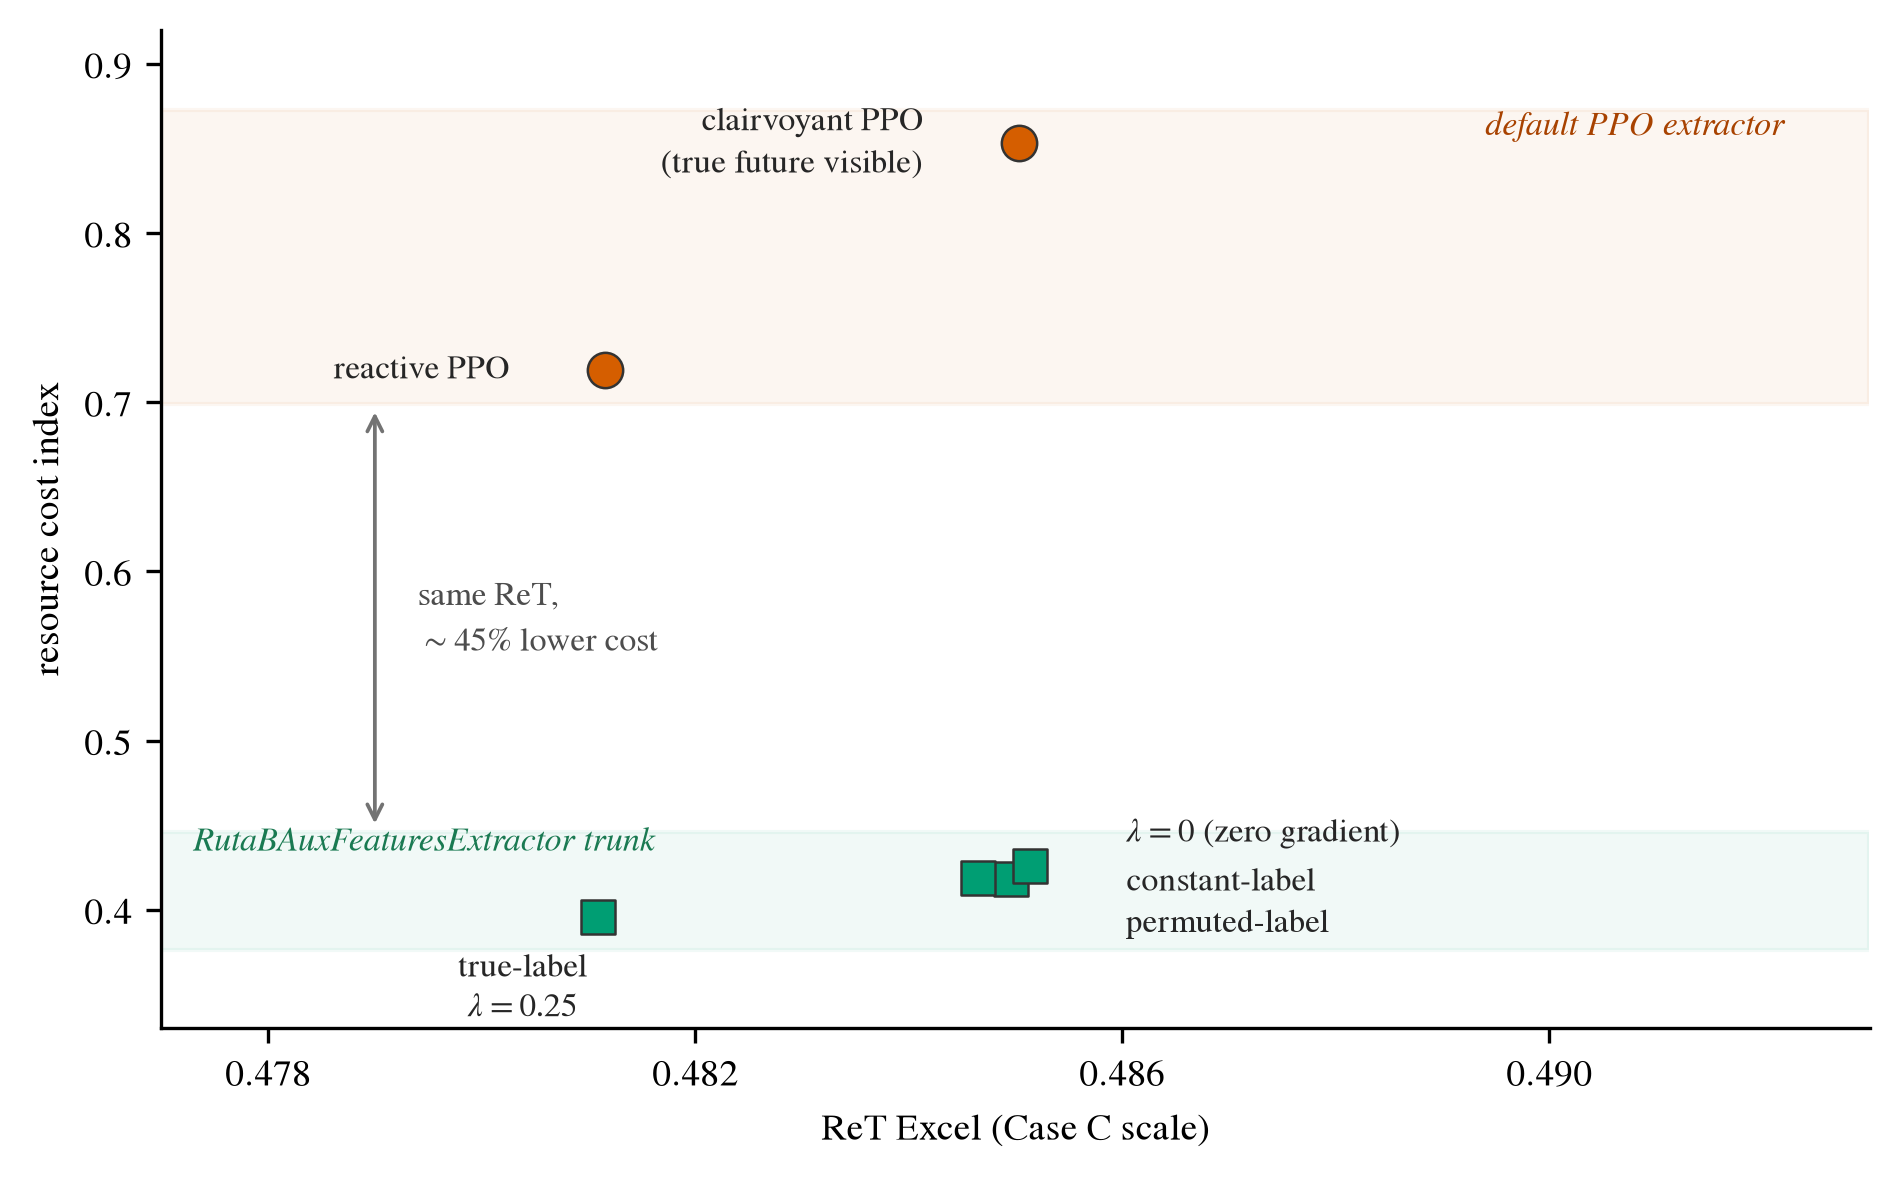
\includegraphics[width=0.85\linewidth]{fig10_efficiency_architecture}
\caption{Efficiency-architecture attribution (control ladder, Case C
downstream-stress scale). The four shared-trunk-extractor arms
(true-label $\lambda{=}0.25$, permuted-label, constant-label, and
$\lambda{=}0$ with zero auxiliary gradient) cluster at cost
$\approx$0.40--0.43 with closely matched Excel ReT, regardless of whether
the auxiliary task carries signal or gradient. The two default-extractor
arms cluster at cost $\approx$0.72--0.85 regardless of foreknowledge.
The cost reduction traces to the extractor architecture, not to
prediction.}
\label{fig:efficiency_architecture}
\end{figure}

\bibliographystyle{elsarticle-num}
\bibliography{references}

\end{document}
